\chapter[Implementación]{
  \label{chp:implementacion}
  IMPLEMENTACIÓN
}
\thispagestyle{numberingStyle}
\pagestyle{numberingStyle}



\section{Estructura de la aplicación}
\subsection{Estructura proyecto Java}
Para la implementación del modelo y la aplicación web, se ha elaborado un proyecto Maven con los siguientes módulos:
\\
\\

\begin{figure}[H]
\centering
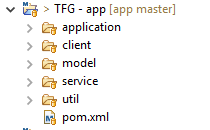
\includegraphics[
   keepaspectratio=true
]{./06_Implementacion/img/estructuraglobaljava.png}
\caption{Estructura proyecto Java}
\end{figure}


\begin{itemize}
	\item \textbf{TFG - app: } Es el proyecto Maven de la aplicación Java. Está formado por diferentes módulos que forman la aplicación:
	\begin{itemize}
		\item \textbf{Application: } Es un módulo donde se encuentran las aplicaciones web del sistema.
		\item \textbf{Client: } Es un módulo donde se implementa el cliente que consume y accede los servicios del modelo. Necesario para la aplicación web.
		\item \textbf{Model: } Donde reside la persistencia y la lógica de negocio de la aplicación.
		\item \textbf{Service : } Es el módulo que define e implementa los servicios.
		\item \textbf{Util : } Módulo de utilidad. Aporta clases y funciones comunes a los demás módulos.
		\item \textbf{pom.xml : } Archivo utilizado por Maven para la construcción del proyecto, manteniendo la gestión de las dependencias y el orden de construcción de los módulos.
	\end{itemize}
\end{itemize}

Con esta separación en módulos conseguimos hacer más independiente cada uno de los módulos que formarán el desplegable de la aplicación. De tal manera, que si queremos utilizar otra implementación de persistencia, simplemente tenemos que reemplazar el JAR generado por dicho módulo por el que queramos utilizar, en el archivo de aplicación web (WAR).

\subsubsection*{Módulo Model}
El módulo \textit{model} de la aplicación está compuesto por: \textit{core} y \textit{persistence}.

\begin{figure}[H]
\centering
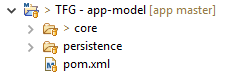
\includegraphics[
   keepaspectratio=true
]{./06_Implementacion/img/estructuramodeljava.png}
\caption{Estructura módulo \textit{model}}
\end{figure}

En el submódulo \textit{persistence} se implementa toda la persistencia de datos, desde las clases persistentes hasta las definiciones e implementaciones de los DAOs. Por su parte, en el submódulo \textit{core} se define e implementa la lógica de negocio.

\subsubsection*{Estructura directorios Model - Persistence}
\begin{figure}[H]
\centering
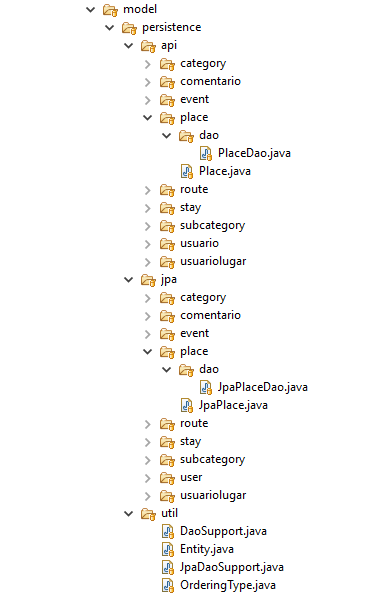
\includegraphics[
   keepaspectratio=true
]{./06_Implementacion/img/estructuramodelpersistence.png}
\caption{Estructura módulo \textit{model-persistence}}
\end{figure}

\begin{itemize}
	\item \textbf{src/main/java/ ../model/persistence/api. } Es el directorio donde se encuentran todas las definiciones de las clases persistentes (Ej: Place.java) y los DAOs (Ej: PlaceDao.java).
	\item \textbf{src/main/java/ ../model/persistence/jpa. } Directorio donde residen las implementaciones de las definiciones anteriores (Ej: JpaPlace.java, JpaPlaceDao.java). Como su nombre indica, se hace uso del API de persistencia JPA. 
	\item \textbf{src/main/java/ ../model/persistence/util. } Es el directorio donde se incluyen clases de utilidad (Ej: DaoSupport y JpaDapSupport, para la implementación de los DAOs).
\end{itemize}

\subsubsection*{Estructura directorios Model - Core}
\begin{figure}[H]
\centering
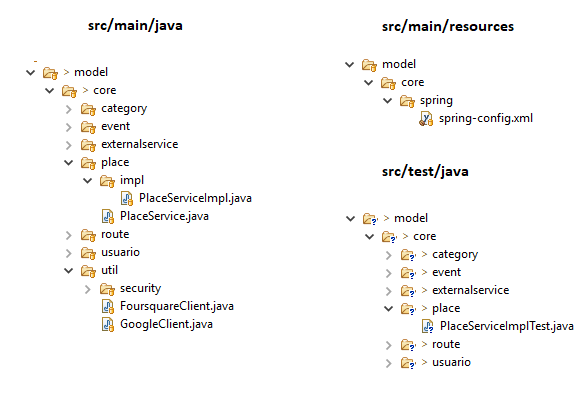
\includegraphics[
   keepaspectratio=true
]{./06_Implementacion/img/estructuramodelcore.png}
\caption{Estructura módulo \textit{model-core}}
\end{figure}

\begin{itemize}
	\item \textbf{src/main/java/ ../model/core. } Directorio donde se especifican e implementan la lógica de negocio de la aplicación.
	\item \textbf{src/main/java/ ../model/core/util. } Directorio de utilidad que incluye los clientes de las APIs externas.
	\item \textbf{src/test/java/ ../model/core. } Incluye las pruebas automatizadas para cada uno de lo servicios de la lógica de negocio.
\end{itemize}


\subsubsection*{Módulo Service}
El módulo \textit{service} de la aplicación está compuesto por los submódulos \textit{api} y \textit{core}.

\begin{figure}[H]
\centering
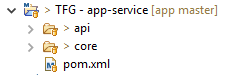
\includegraphics[
   keepaspectratio=true
]{./06_Implementacion/img/estructuraservice.png}
\caption{Estructura módulo \textit{service}}
\end{figure}


\subsubsection*{Estructura directorios Service - Api}
\begin{figure}[H]
\centering
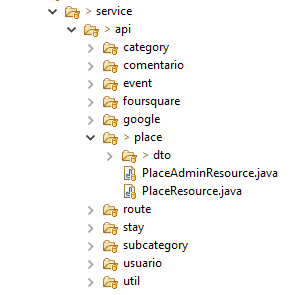
\includegraphics[
   keepaspectratio=true
]{./06_Implementacion/img/estructuraserviceapi.png}
\caption{Estructura módulo \textit{service-api}}
\end{figure}

\begin{itemize}
	\item \textbf{src/main/java/ ../service/api. } Directorio donde se definen cada uno de los recursos web, siguiendo la API de JAX-RS que ofrece el soporte para la creación de servicios web, que ofrecerán remotamente, los servicios de la capa modelo. Se puede observar la definición dos recursos web, como son: \textit{PlaceResource.java} y \textit{PlaceAdminResource.java}.
\end{itemize}


\subsubsection*{Estructura directorios Service - Core}
\begin{figure}[H]
\centering
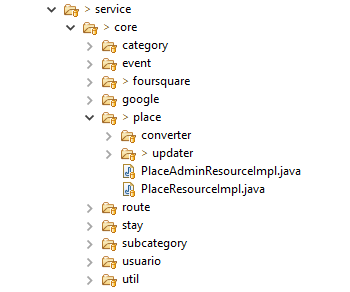
\includegraphics[
   keepaspectratio=true
]{./06_Implementacion/img/estructuraservicecore.png}
\caption{Estructura módulo \textit{service-core}}
\end{figure}

\begin{itemize}
	\item \textbf{src/main/java/ ../service/core. } Directorio con las implementaciones para cada uno de los recursos definidos en el submódulo \textit{service-api}. Se puede observar las clases \textit{PlaceResourceImpl.java} y \textit{PlaceAdminResourceImpl.java} que implementa las clases mostradas en el submódulo anterior.
	\begin{itemize}
		\item \textbf{../service/core/*/converter. } Directorio con las clases necesarias para la conversión de objetos a persistentes a objetos de transferencia de datos.
		\item \textbf{../service/core/*/updater. } Directorio con las clases necesarias para la creación del objeto persistente a modificar a partir del objeto de transferencia de datos recibido. 
		\item \textbf{../service/core/util. } Directorio en el que se encuentran clases que ofrecen funcionalidades como la conversión de excepciones Java a respuestas HTTP, validadores de datos de entrada, etc...
	\end{itemize}
\end{itemize}



\subsubsection*{Módulo Application}
\begin{figure}[H]
\centering
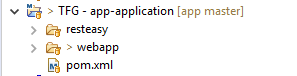
\includegraphics[
   keepaspectratio=true
]{./06_Implementacion/img/estructuraapplication.png}
\caption{Estructura módulo \textit{application}}
\end{figure}

Formado por los submódulos \textit{resteasy} y \textit{webapp}. El primero de ellos será el encargado de ofrecer una aplicación REST, donde se expondrán remotamente, los servicios creados en la capa de servicios del modelo. Utilizará el proyecto \textit{JBoss RESTEasy} como implementación del API de JAX-RS.

Por su parte, el módulo \textit{webapp} será el encargado de ofrecer una aplicación web, accesible mediante navegador web. Seguirá una arquitectura MVC.


\subsubsection*{Estructura directorios Application - Resteasy}
\begin{figure}[H]
\centering
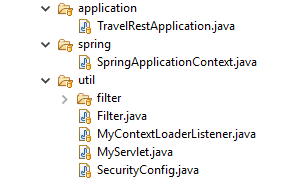
\includegraphics[
   keepaspectratio=true
]{./06_Implementacion/img/estructuraapplicationresteasy.png}
\caption{Estructura módulo \textit{application-resteasy}}
\end{figure}

\begin{itemize}
	\item \textbf{src/main/java/ ../application/resteasy. }
	\begin{itemize}
		\item \textbf{../application/resteasy/application. } Directorio con la clase encargada de añadir al contenedor de la aplicación los objetos definidos en la capa de servicios.		
		\item \textbf{../application/resteasy/filter. } Directorio en el que se encuentran los filtros de la aplicación.
		\item \textbf{../application/resteasy/spring. } Directorio con la clase encargada de obtener los objetos del contenedor de Spring y poder incorporarlos al contenedor de la aplicación. para su uso.
	\end{itemize}
\end{itemize}



\subsubsection*{Estructura directorios Application - Webapp}
\begin{figure}[H]
\centering
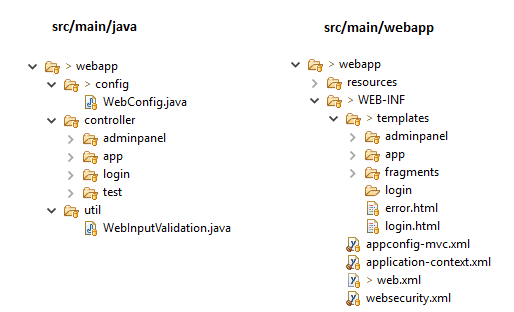
\includegraphics[
   keepaspectratio=true
]{./06_Implementacion/img/estructuraapplicationwebapp.png}
\caption{Estructura módulo \textit{application-resteasy}}
\end{figure}

\begin{itemize}
	\item \textbf{src/main/java. }
	\begin{itemize}
		\item \textbf{../application/webapp/config. } Directorio donde residen archivos de configuración de la aplicación.
		\item \textbf{../application/webapp/controller. } Directorio en el que se encuentran implementados los controladores de la aplicación.
		\item \textbf{../application/webapp/util. } Directorio con las clases de utilidad.
	\end{itemize}
	\item \textbf{src/main/webapp. }
	\begin{itemize}
		\item \textbf{../application/webapp/resources. } Directorio con los ficheros que aportan un mejor aspecto a la web. Incluye, archivos JavaScript, CSS e imágenes.
		\item \textbf{../application/webapp/WEB-INF. } Directorio en el que se encuentran las plantillas HTML utilizadas para crear las páginas web.
	\end{itemize}
\end{itemize}


\subsubsection*{Módulo Client}
\begin{figure}[H]
\centering
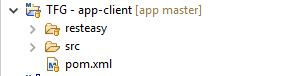
\includegraphics[
   keepaspectratio=true
]{./06_Implementacion/img/estructuraclient.png}
\caption{Estructura módulo \textit{client}}
\end{figure}

El módulo \textit{client} está compuesto, únicamente, del módulo \textit{resteasy}. Este módulo, define e implementa un cliente para la aplicación REST anteriormente comentada.


\subsubsection*{Estructura directorios Client - Resteasy}
\begin{figure}[H]
\centering
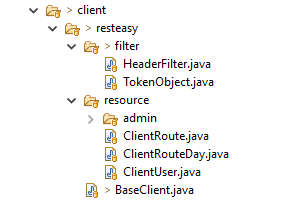
\includegraphics[
   keepaspectratio=true
]{./06_Implementacion/img/estructuraclientresteasy.png}
\caption{Estructura módulo \textit{client-resteasy}}
\end{figure}

\begin{itemize}
	\item \textbf{src/main/java/ ../client/resteasy. }
	\begin{itemize}
		\item \textbf{../resteasy/filter. } Directorio donde residen los filtros utilizados por el cliente.
		\item \textbf{../resteasy/resource. } Directorio en el que se encuentran implementados los clientes específicos para cada servicio.
	\end{itemize}
\end{itemize}


\subsection{Estructura proyecto Ionic}


\section{Implementación capa modelo}


\subsection{Persistencia}


\subsection{Acceso a datos}


\subsection{Gestión de la transaccionalidad}


\section{Implementación capa servicios}


\section{Implementación autenticación y autorización}


\section{Implementación cliente web}


\section{Implementación cliente móvil}
